\chapter{Methodology}
\label{cap:methodology}

This chapter will address the definition and justification of the working methodology used, as well as the planification of the project. The technological resources and tools employed will also be exposed in detail.

\section{Agile methodologies}
\label{sec:agileMethodologies}

The Agile Manifesto \cite{agile_manifesto} was born in 2001 as a set of four values and twelve principles associated with the search for improvements in software development over conventional methodologies. In this manifesto, the assessments of expert software practitioners were declared, stating the importance of:

\begin{itemize}
\item Individuals and interactions over processes and tools.
\item Working software over comprehensive documentation.
\item Customer collaboration over contract negotiation.
\item Responding to change over following a plan.
\end{itemize}

Agile methodologies promote the continuous delivery of software in short cycles, fostering involvement, training and adjustment to stakeholders needs \cite{mora_conversaciones_2017}. These methodologies mean, in turn, greater flexibility, increased productivity and, consequently, cost reductions during changing projects, where the requirements can differ throughout their development.

Nowadays, the benefits associated with agile methodologies have made them widely used by practitioners, enhancing the perceived and internal quality of software development as well as promoting their profitability.

\section{OpenUP}
\label{sec:openUP}

Being aware of the advantages associated with the use of agile methodologies in software engineering and given the iterative and incremental nature of this project, the methodology chosen for its development was OpenUP \cite{macisaac_eclipse}. 

OpenUp is a minimum and sufficient methodology, which means that it only considers the fundamental contents of software development, leaving aside aspects such as the management of large teams, technology-specific guidance or contractual situations. In spite of its simplicity, OpenUP covers in a complete and agile way the whole development process of a software project, being completely flexible to the nature of the project in which it is employed.

The main principles of OpenUP offer a direct mapping with the ones expressed in the agile manifesto and try to represent the working model to follow by using this methodology:

\begin{itemize}
\item \textbf{Collaborate to align interest and share understanding}, advocating for coordination and mutual understanding among stakeholders.

\item \textbf{Balance competing priorities to maximize stakeholder value}, trying to maximize profits while conforming to project constraints.

\item \textbf{Focus on the architecture early to minimize risks and organize development}.

\item \textbf{Evolve to continuously obtain feedback and improve}, in order to have continuous communication with stakeholders and demonstrate incremental value to them.

\end{itemize}

\section{Phases and project planning}
\label{sec:phasesAndPlanning}

The use of agile, iterative, and incremental methodologies such as OpenUP facilitates the coordination and development of projects based on multiple modules that, once developed, add value to the desired final product.

As shown in Fig.~\ref{fig:openUP}, the organisation of work followed by OpenUP distinguishes between three different perspectives based on personal, team and stakeholder levels:

\begin{figure}[htb]
	\centering
	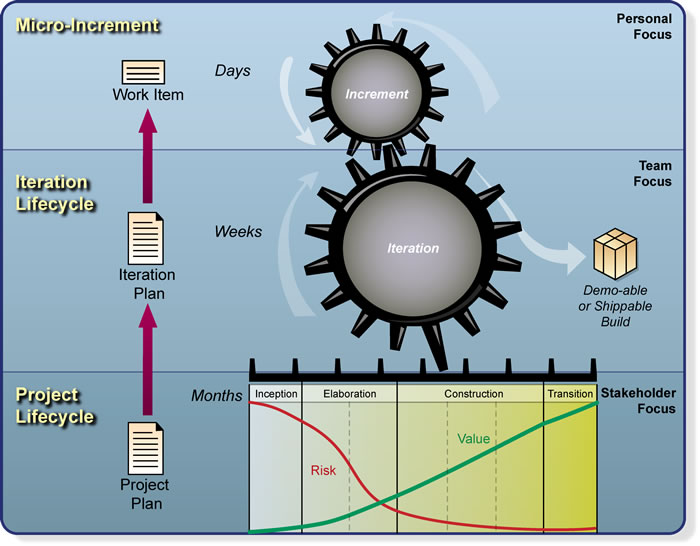
\includegraphics[width=0.8\linewidth]{3_openup}
	\caption[OpenUP lifecycle]{OpenUP lifecycle layers (source: \url{https://www.ida.liu.se/~TDDD77/openup/index.htm})}
	\label{fig:openUP}
\end{figure}

\begin{itemize}
\item The personal effort of an OpenUP project is defined as a \textbf{micro-increment}, commonly measured in hours or days.

\item From the team’s perspective, an \textbf{iteration lifecycle} reflects how micro-increments are applied to obtain stable and cohesive builds of the system being produced.

\item Focusing on how an overview of the project is guaranteed for the stakeholders, OpenUP structures the \textbf{project lifecycle} into four phases: \emph{Inception}, \emph{Elaboration}, \emph{Construction}, and \emph{Transition}.
\end{itemize}

%%%%%%%%%%%%%%%%%%%%%%%%%%%%%%%%%%%5

Thus, each of the phases of the OpenUP lifecycle are defined as follows:

\begin{itemize}

\item \textbf{Inception phase}: in this phase, it is a question of understanding what is intended to be produced and what are the objectives and limitations of the system to be developed, identifying the stakeholders, and detailing their success criteria.

\item \textbf{Elaboration phase}: it involves the procurement of a more detailed understanding of the system requirements; design, implementation, validation and establishment of the architecture baseline, providing a skeleton of the system structure; mitigation of essential risks and project planning in terms of time and costs.

\item \textbf{Construction phase}: iterative development of the desired product, until a tested result is achieved and ready to be offered to users. The goal pursued during this phase is to minimize costs through resource optimization and parallelization of independent tasks.

\item \textbf{Transition phase}: this last phase involves validating user expectancies, obtaining stakeholders approval, and seeking to improve future projects based on well-documented lessons learned.

\end{itemize}

These phases, applied to the particular case of this project, are presented in the following way:

\subsection{Inception phase}
\label{sec:inceptionPhase}

In this phase, the justification of the project was carried out, identifying its scope and the objectives to be pursued. Its feasibility in terms of risks, time and estimated costs was also assessed. Roles were assigned and, at the same time, an attempt was made at identifying the key functionalities of the system in accordance with the specifications defined with the identified stakeholders.

At this stage, the first meetings were held to establish the key functionalities of the system, to understand the competencies addressed and to provide an insight into how to proceed in the months ahead.

\subsection{Elaboration phase}
\label{sec:elaborationPhase}

Once an overview of the project had been established, a more detailed understanding of the objectives pursued was sought in this phase. To perform this task, a series of interviews with the stakeholders were planned and conducted, allowing to know the essential features that the system should meet. On this basis, the elicitation and formalised documentation of the system's requirements was carried out, allowing to proceed with the analysis and design of the functional modules that would compose the system.

Other tasks inherent to this stage were addressed, such as the choice of technological resources to be used, the development process employed, the definition of the system architecture baseline or the acquisition of domain-specific knowledge. Actors and use cases were also formally defined.

Finally, considering the set of formally stated requirements as well as the resulting skeleton of the system to be developed, a project planning consisting of time and cost estimation was elaborated. Based on the identified functionalities, the iterations that constitute the lifecycle were organized according to the priorities expressed by the stakeholders.

\subsection{Construction phase}
\label{sec:constructionPhase}

In this stage, the implementation of the different functionalities of the system was carried out. This implementation was undertaken in an orderly manner based on the priorities agreed upon with the stakeholders in the previous phase.

Presented in priority order, the following system functionalities were developed:

\begin{itemize}
\item \textbf{Module 1}: API skeleton. 
\item \textbf{Module 2}: Main user interface.
\item \textbf{Module 3}: STC measurement.
\item \textbf{Module 4}: Data visualization.
\item \textbf{Module 5}: Recommendation system.
\item \textbf{Module 6}: Settings and preferences.
\end{itemize}

The implementation of each module was done in an iterative way, trying to agree with the stakeholders (the project tutors) any kind of modification in the functionality or the interface considered during this development stage. As would be reflected in the planning, each functional module was associated with an iteration during the construction phase of the project.

\subsection{Transition phase}
\label{sec:transitionPhase}

Finally, the transition stage was dedicated to the documentation, testing and deployment of the system, confirming compliance with the requirements with the stakeholders and elaborating the final project report.

The review of the project by the tutors as well as the preparation of the project presentation were also part of this stage.

\section{Roles}
\label{sec:roles}

In this subsection, the set of basic OpenUP roles will be defined as well as the assignment of those roles for the concrete case of this project.

\begin{itemize}
\item \textbf{Analyst}: is the person in charge of identifying and understanding the problems and opportunities of the project, by knowing and interpreting the requirements expressed by the customer and end-users.

\item \textbf{Architect}: designs and documents the system architecture, being responsible for technical decisions on the overall implementation of the system.

\item \textbf{Developer}: each person in this role is responsible for the implementation of a set of parts of the system, adjusting it to the architecture and using the necessary technologies for the development.

\item \textbf{Project manager}: is the person in charge of planning the project, fulfilling the objectives as well as communicating and coordinating with the stakeholders.

\item \textbf{Tester}: person in charge of the identification, definition, implementation and execution of the tests over the system.

\item \textbf{Stakeholders}: people that may be directly or indirectly affected by project realization. Normally a stakeholder is a person whose needs will be met after the project is completed, like end-users o customers.
\end{itemize}

The general assignment of the OpenUP roles for this project is detailed in Table~\ref{tb:roles}.

\begin{table}[htb]
	\centering
	\caption[Roles assignment]{Roles assignment}
	\label{tb:roles}
	\begin{tabular}{|c|c|c|}
	\hline
	\textbf{Role}   & \textbf{Person}                           & \textbf{Charge}                  \\ \hline\hline
	Analyst         & \multirow{5}{*}{Antonio Manjavacas Lucas} & \multirow{5}{*}{Grade student}   \\ \cline{1-1}
	Architect       &                                           &                                  \\ \cline{1-1}
	Developer       &                                           &                                  \\ \cline{1-1}
	Project manager &                                           &                                  \\ \cline{1-1}
	Tester          &                                           &                                  \\ \hline
	Stakeholder     & Aurora Vizcaíno Barceló                   & Project supervisor and professor \\ \hline
	Stakeholder     & José Ángel Olivas Varela                  & Project supervisor and professor \\ \hline
	\end{tabular}
\end{table}


On the one hand, Aurora Vizcaíno was in charge of monitoring and providing feedback on the project: due to her experience in the field of GSD, she elicited the key requirements of the system, served as a guide throughout its planning and development and acted as a contact person for any queries during the project.

On the other hand, José Ángel Olivas was responsible for recommending and guiding the implementation of the modules related to the competencies of the Computing intensification, such as the underlying fuzzy logic mechanisms used to describe the communications and coordination between users by the expert system.

Finally, the tasks of analysis, design, development, testing, and documentation were carried out by Antonio Manjavacas, the grade student responsible for the project.

\section{Resources}
\label{sec:resources}

The following sub-sections will detail the hardware and software resources used in the development of this project.

\subsection{Hardware resources}
\label{sec:hardwareRes}

The hardware resources used are shown below:

\begin{itemize}
\item \href{https://www8.hp.com/}{HP} Pavilion x360 Convertible 14-cd0xxx equipped with:
	\begin{itemize}
	\item Intel(R) Core(TM) i7-8550U CPU @ 1.80GHz 1.99GHz, 64 bits
	\item 12 GB RAM
	\item Integrated graphics Intel(R) UHD Graphics 620
	\item NVIDIA GeForce MX130
	\end{itemize}
\end{itemize}

\subsection{Software resources}
\label{sec:softwareRes}

Likewise, these were the technologies, environments and programming languages used throughout the project:

\begin{itemize}

\item \href{https://www.java.com/}{Java 1.8}. General purpose, high level, object-oriented programming language. It is one of the most widely used programming languages by the developers community nowadays. Java stands out for its ease of learning and use, as well as its security and portability to any device capable of running Java Virtual Machine (JVM).\newline

\item \href{https://maven.apache.org/}{Apache Maven}. Tool for the management and automation of Java projects, facilitating dependencies management and software building. It is maintained by the Apache Software Foundation and is widely used by the Java community.\newline

\item \href{https://git-scm.com/}{Git}. Distributed version control system based on repositories. Facilitates version, branch, and data integrity management in software projects.\newline

\item \href{https://github.com/}{GitHub}. Hosting system for version control using Git. It facilitates the management of repositories and projects, offering multiple facilities in their creation and maintenance.\newline
	
\item \href{https://spring.io/}{Spring Framework}. Framework for the development of Java applications developed by Pivotal Software. It provides easy integration with Maven and other services to achieve the development of web applications.\newline

\item \href{https://www.mongodb.com/}{MongoDB}. Database management system, NoSQL and document based. Chosen for its easy use and optimization for the treatment of large data sets. Provides an easy integration with the rest of the tools employed, such as Spring framework.\newline
	
\item \href{https://www.mongodb.com/cloud/atlas/}{MongoDB Atlas}. MongoDB cloud database hosting service. It offers limited free storage as well as an easy connection and usage by applications via URI.\newline

\item \href{https://www.eclipse.org/ide/}{Eclipse}. Integrated Development Environment (IDE) widely used in Java development, among other languages. 
It includes utility plugins that facilitate integration with Git (\href{https://www.eclipse.org/egit/}{EGit}) or Maven (\href{https://www.eclipse.org/m2e/}{m2Eclipse}).\newline

\item \href{https://code.visualstudio.com/}{Visual Studio Code}. Free and open source code editor, which offers a large number of plugins and language support.\newline

\item \href{https://www.python.org/}{Python}. Interpreted, multi-paradigm, dynamic and multi-platform programming language. It stands out for its readability and usability.\newline

\item \href{http://jfuzzylogic.sourceforge.net/html/index.html}{jFuzzyLogic}. Java library for handling and working with fuzzy logic \cite{cingolani_jfuzzylogic_2012,cingolani_jfuzzylogic_2013}. It is based on the standard FCL (Fuzzy Control Language) and is freely distributed.\newline

\item \href{http://ffll.sourceforge.net/fcl.htm}{FCL}. Fuzzy Control Language published by the International Electrotechnical Commission (IEC). It is specified in the IEC 61131-7 document and allows the standardization of fuzzy control systems.\newline

\item \href{https://www.w3.org/html/logo/}{HTML 5}. Markup language used in web development. It is a standard in charge of the World Wide Web Consortium (W3C) and is currently in its version 5.\newline

\item \href{https://www.w3.org/Style/CSS/Overview.en.html}{CSS}. These cascading style sheets constitute a graphic design language used in conjunction with markup languages such as HTML. Used to enhance the appearance of user interfaces and customize their appearance.\newline
	
\item \href{https://getbootstrap.com/}{Bootstrap}. Open source multi-platform library for frontend design. It offers design templates based on HTML, CSS, and JavaScript.\newline

\item \href{https://www.javascript.com/}{JavaScript}. Interpreted, object-oriented, prototype-based, imperative, weakly typed and dynamic programming language. Widely used in client-side web development.\newline

\item \href{https://www.chartjs.org/}{Chart.js}. Open source JavaScript library for creating graphics and animations in HTML5.\newline

\item \href{https://jquery.com/}{jQuery}. JavaScript library aimed to simplify interaction with HTML and make client-side AJAX  (Asynchronous JavaScript And XML) requests in web applications.\newline

\item \href{https://www.postman.com/}{Postman}. A tool for the creation of API requests in a simple and fast way. It eases the testing of web applications and allows a high customization of the requests.\newline

\item \href{https://www.heroku.com/}{Heroku}. Cloud Computing Platform as a Service (PaaS). Enables deployment of cloud applications and offers limited free hosting.\newline

\item \href{https://ubuntu.com/}{Ubuntu}. Free and open-source Linux distribution distributed by Canonical Ltd. Used in the deployment procedure and part of the application development.\newline

\item \href{https://www.microsoft.com/en-us/windows/}{Windows 10}. Operating system developed and distributed by Microsoft. Used in most of the application development.\newline

\item \href{https://www.zotero.org/}{Zotero}. Free and open bibliographic reference manager. It is multi-platform and offers a browser extension that facilitates the management and collection of references.\newline

\item \href{https://www.latex-project.org/}{\LaTeX}. Markup language oriented to the elaboration and layout of high-quality documents. Based on \TeX, initially developed by Donald Knuth. The template available in \cite{salidoTFGgit} has been used to elaborate this document.\newline
	
\item \href{https://www.texstudio.org/}{{\TeX}studio}. Integrated writing IDE for creating \LaTeX documents. {\TeX}studio is open source and available for all major operating systems.\newline

\item \href{https://www.microsoft.com/en-us/microsoft-365/word/}{Microsoft Word}. WYSIWYG text editor distributed by Microsoft in its Microsoft Office package. Used for the elaboration of the draft memory and basic documental tasks during the project.\newline

\item \href{https://www.microsoft.com/en-us/microsoft-365/onedrive/online-cloud-storage/}{Microsoft OneDrive}. Cloud data storage system offered by Microsoft. Used for the storage of documents, backups, code, and diagrams.\newline

\item \href{https://www.diagrams.net/}{Diagrams.net}. Previously known as Draw.io, it is a tool for creating diagrams and charts. It is open source and offers online and desktop support.\newline

\end{itemize}

Finally, a summary of the software resources used is shown in Fig.~\ref{fig:swResources}.

\begin{figure}[htb]
	\centering
	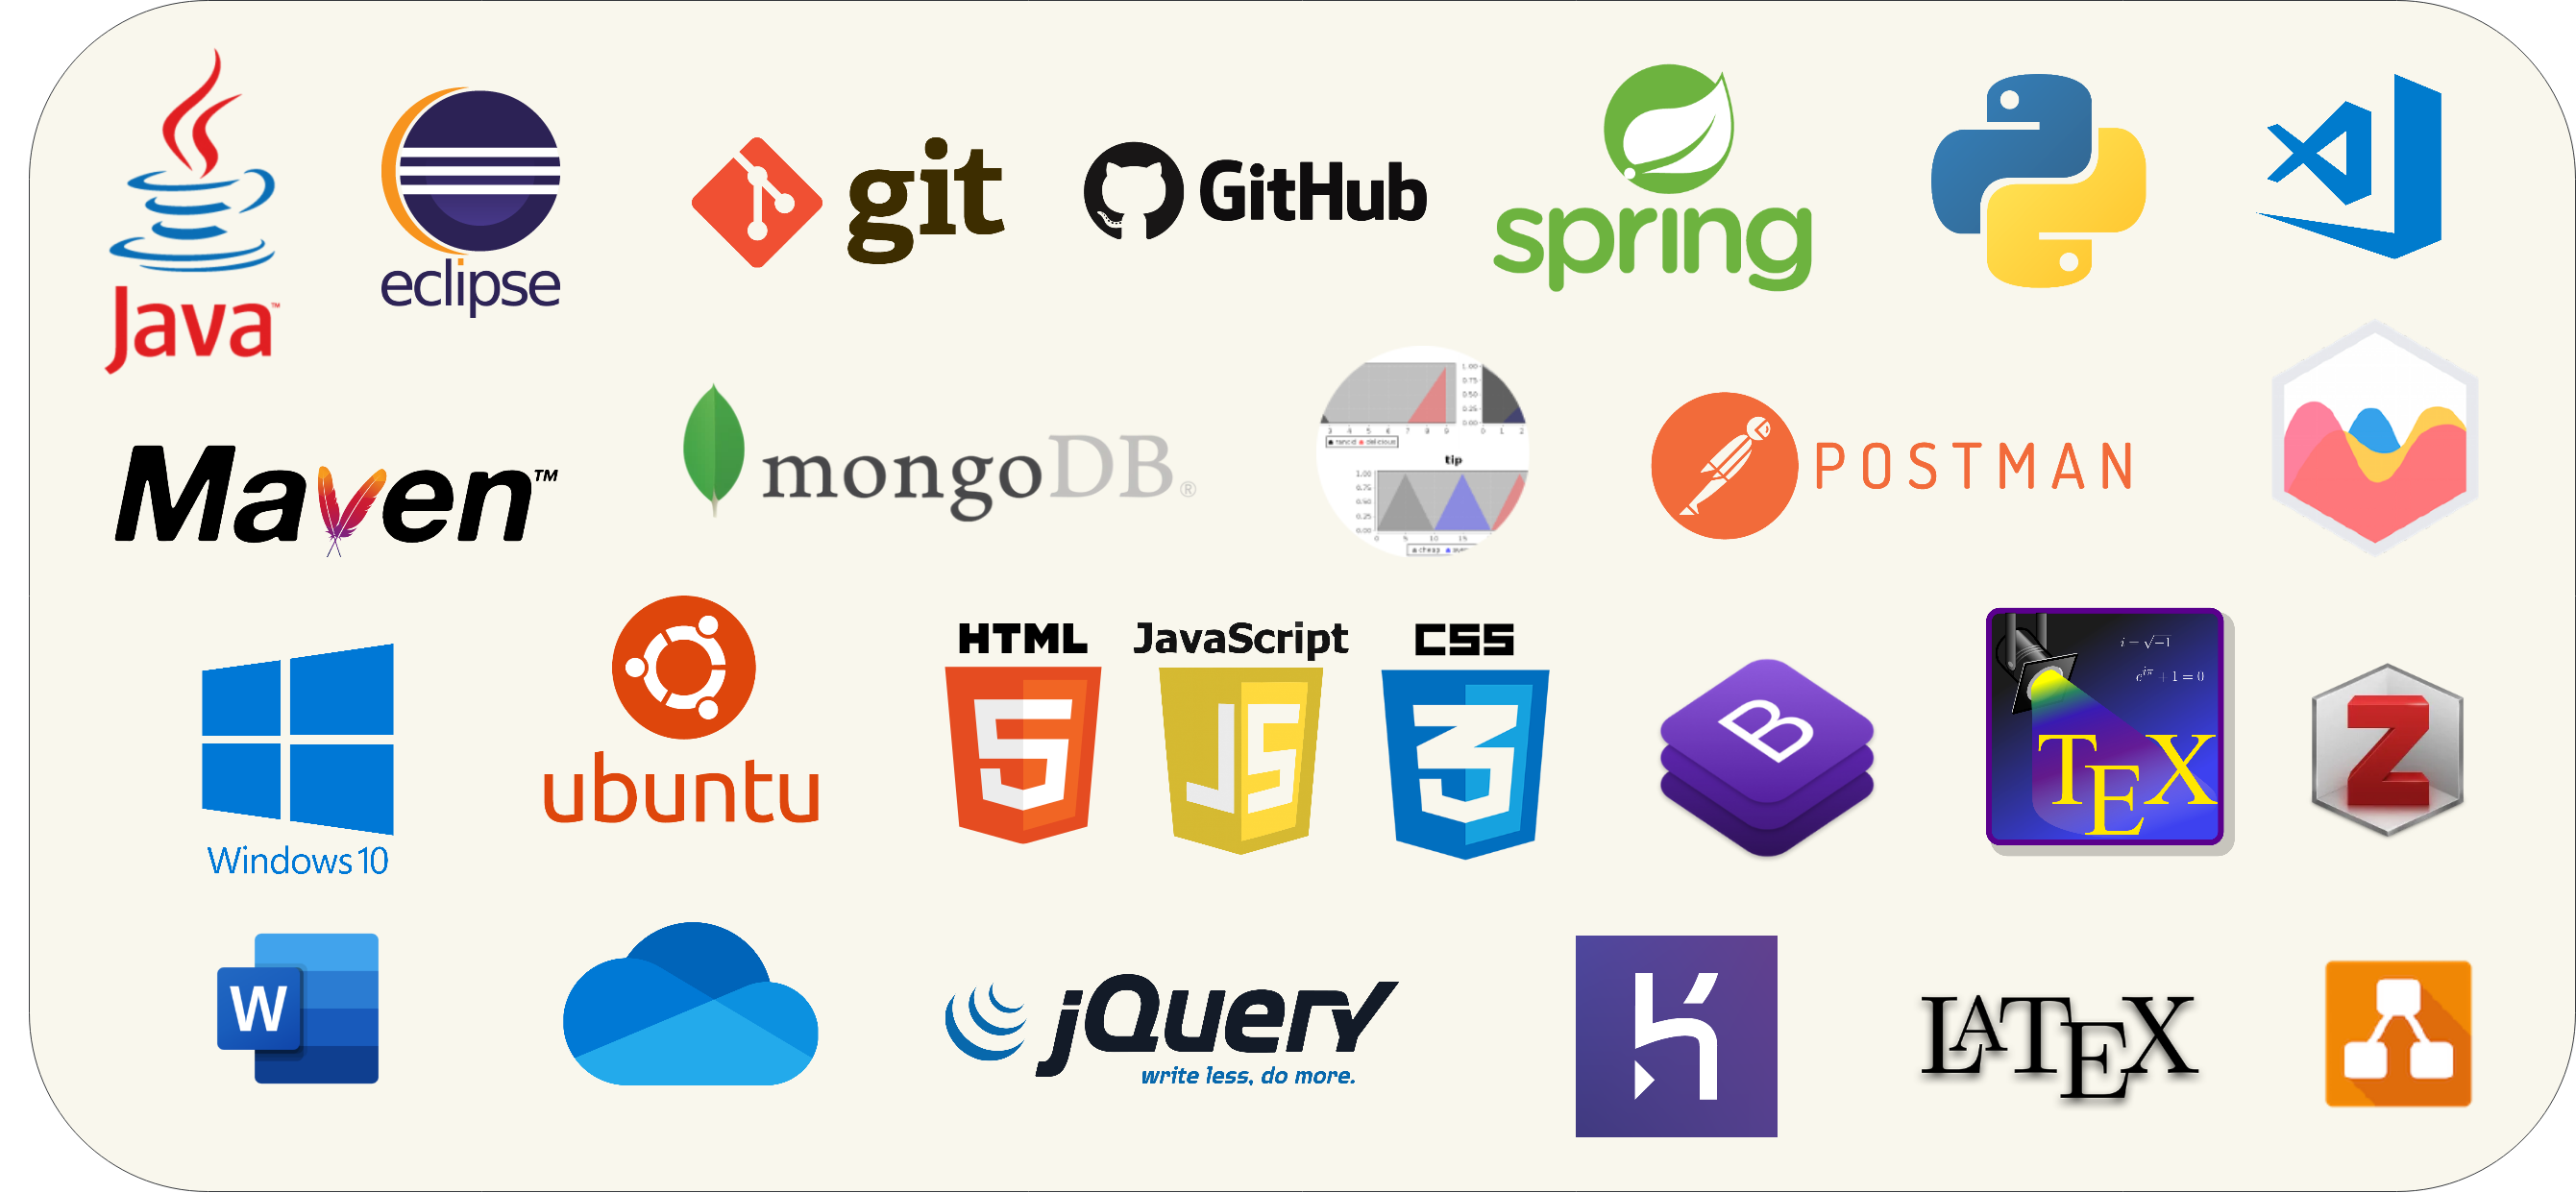
\includegraphics[width=0.9\linewidth]{3_tools}
	\caption[Software resources]{Software resources used in this project}
	\label{fig:swResources}
\end{figure}


